% \iffalse
\let\negmedspace\undefined
\let\negthickspace\undefined
\documentclass[journal,12pt,twocolumn]{IEEEtran}
\usepackage{cite}
\usepackage{amsmath,amssymb,amsfonts,amsthm}
\usepackage{algorithmic}
\usepackage{graphicx}
\usepackage{textcomp}
\usepackage{xcolor}
\usepackage{txfonts}
\usepackage{listings}
\usepackage{enumitem}
\usepackage{mathtools}
\usepackage{gensymb}
\usepackage{comment}
\usepackage[breaklinks=true]{hyperref}
\usepackage{tkz-euclide} 
\usepackage{listings}
\usepackage{gvv}                                        
\def\inputGnumericTable{}                                 
\usepackage[latin1]{inputenc}                                
\usepackage{color}                                            
\usepackage{array}                                            
\usepackage{longtable}                                       
\usepackage{calc}                                             
\usepackage{multirow}                                         
\usepackage{hhline}                                           
\usepackage{ifthen}                                           
\usepackage{lscape}
\usepackage{pgfplots}

\newtheorem{theorem}{Theorem}[section]
\newtheorem{problem}{Problem}
\newtheorem{proposition}{Proposition}[section]
\newtheorem{lemma}{Lemma}[section]
\newtheorem{corollary}[theorem]{Corollary}
\newtheorem{example}{Example}[section]
\newtheorem{definition}[problem]{Definition}
\newcommand{\BEQA}{\begin{eqnarray}}
\newcommand{\EEQA}{\end{eqnarray}}
\newcommand{\define}{\stackrel{\triangle}{=}}
\theoremstyle{remark}
\newtheorem{rem}{Remark}
\begin{document}

\bibliographystyle{IEEEtran}
\vspace{3cm}

\title{NCERT-Analog-11.15-6}
\author{EE22BTECH11004 - Allu lohith}

\maketitle
\newpage
\bigskip

\renewcommand{\thefigure}{\theenumi}
\renewcommand{\thetable}{\theenumi}
\begin{enumerate}
\item A bat emits ultrasonic sound of frequency $1000 kHz$ in air. If the sound meets a water surface, what is the wavelength of\\[0pt] \brak the reflected sound \\[0pt]
\brak{b} the transmitted sound?\\
Speed of sound in air is $340 ms^{-1}$ and in water is $1486 ms^{-1}$.\\
\item[Soln:]


\setlength{\intextsep}{2pt}
\begin{table}[h!]
\centering
\renewcommand{\arraystretch}{2}
\begin{tabular}{|c|c|c|}
\hline 
\setlength{\tabcolsep}{1pt}
\textbf{Parameter}  &\textbf{Description} &\textbf{Formulae/Value} \\
\hline
$a\brak 0$ & First term of A.P & - \\
\hline
\textbf{$d$} & Commom difference & - \\
\hline
n & Count of terms starting from '0' & - \\
\hline
$a\brak n$ & $(n+1)^{th}$ term of the A.P & $a\brak0 + nd$ \\
\hline
$a\brak{21}$ & Value of $22^{nd}$ term & 149 \\

\hline
$S\brak n$ & Sum of (n+1) terms in A.P & $\left(\frac{n+1}{2}\right) (2a\brak0+nd)$ \\
\hline
\end{tabular}

\vspace{0.5cm}
\caption{\normalsize $Parameters$}
\label{tab:parameters}
\end{table}

The frequency of sound does not change with medium. And,
\begin{align}
{\lambda}\cdot {\text{f}}={\text{v}}
\end{align}

So,
\begin{align}
\lambda_w=v_w/ \text{f}\\
\lambda_w=1486/1000KHz\\
\lambda_w=1.486mm    
\end{align}

\begin{align}
\lambda_a=v_a/\mathrm{f}\\
\lambda_a=340/1000KHz\\
\lambda_a=0.34mm    
\end{align}

The general equation of a sound wave is
\begin{align}
y\brak{t}=A \sin (2\pi\text{f} t-kx)
\end{align}

\begin{table}[h!]
\centering
\renewcommand{\arraystretch}{2}
\begin{tabular}{|c|p{2cm}|}
\hline 
\textbf{Parameter}  &\textbf{Description}  \\
\hline
f & Frequency of sound   \\
\hline
$A$ & Amplitude of the wave   \\
\hline
$t$ & Time \\
\hline
$x$ & Position  \\
\hline
$y(t)$ & Position of particle as a function of time\\
\hline
\end{tabular}

\vspace{0.5cm}
\label{tab:Parameters}
\end{table}


\begin{align}
    K_a=\left(\dfrac{0.34\times 10^{-3}}{2 \times 3.14 }\right)\\
    K_a=54 \times 10^{-6} \: m^{-1}
\end{align}
\begin{align}
    K_w= \left(\frac{1.486 \times 10^{-3}}{2 \times 3.14}\right)\\
    K_w=236 \times 10^{-6} \: m^{-1}
\end{align}\\
\setlength{\intextsep}{2pt}
\begin{table}[h!]
\centering
\begin{tabular}{|c|p{2cm}|c|c|}
\hline 
\textbf{Parameter}  &\textbf{Description} &\textbf{Formula} &\textbf{value} \\
\hline
$\lambda_a$ & Wave length of the reflected sound & $v_a/\text{f}$& $0.34mm$  \\
\hline
$\lambda_w$ &  Wave length of the reflected sound & $v_w/\text{f}$ &$1.486mm$ \\
\hline
\end{tabular}

\vspace{0.5cm}
\caption{\normalsize $Results$}
\label{tab:parameters}
\end{table}
\begin{align}
    y \brak{t}_{Air}=A \sin (6.28 \times 10^{6} t-54\times 10^{-6}x)
\end{align}
\begin{align}
    y \brak{t}_{Water}=A \sin (6.28 \time 10^{6}t - 236 \times 10^{-6}x)
\end{align}\\
\\

\end{enumerate}


\begin{table}[h!]
\centering
\renewcommand{\arraystretch}{2}
\begin{tabular}{|c|p{2cm}|c|c|c|}
\hline 
\textbf{Parameter}  &\textbf{Description} &\textbf{Formula}& \textbf{Variables} & \textbf{Variables Description}\\ 
\hline
V & Speed of sound  & $\sqrt{ \dfrac{\gamma \cdot P}{\rho}} $ & $\gamma$&adiabatic index  \\
 \cline{4-5}
&&& V & Speed of sound\\
 \cline{4-5}
&&& $P$ & Pressure of Medium \\
\cline{4-5}
&&& $\rho$ & Density of medium\\ 
\hline
\end{tabular}

\vspace{0.5cm}
\caption{\normalsize General Equation of speed of sound}
\label{tab:General Equation of speed of sound}
\end{table}



\begin{figure}[h]
    \centering

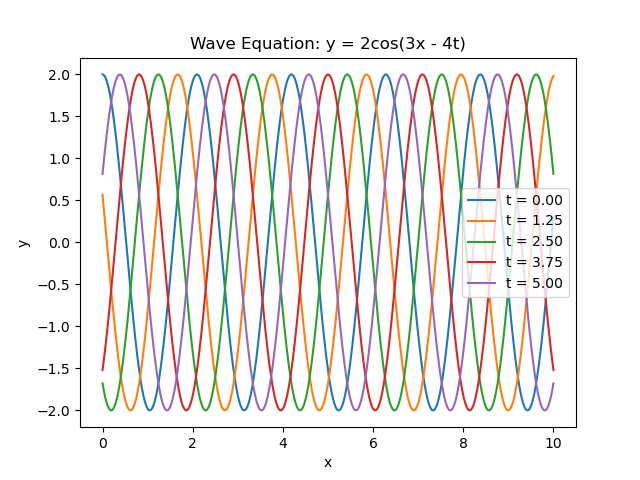
\includegraphics[width=\columnwidth]{graph.png}

\begin{center}
    \caption{A Sound wave}
\end{center}
    
    \label{fig:Sound Wave}
\end{figure}

\end{document}
